\section*{Thresholding}

Also known as \textbf{binarization}; grayscale $\rightarrow$ binary
image, where each pixel is either black or white

\section*{Single Value Thresholding}

\begin{equation*}
  g(x,y) =
  \begin{cases}
    1, & \text{if } f(x,y) > T,\\
    0, & \text{if } f(x,y) \le T.
  \end{cases}
\end{equation*}

\subsection*{Basic Global Thresholding}

Partitions the \textbf{histogram} of an image using a single global
threshold; success depends on how well the histogram can be separated
into two distinct peaks.

\begin{algorithm}[ht]
  \SetAlgoLined
  \DontPrintSemicolon
  Select an initial estimate for $T$ (typically the average grey
  level in the image)\;
  \Repeat{\textnormal{the difference in} $T$ \textnormal{in
      successive iterations is less than
  a predefined limit} $T_{\infty}$}{
    Segment the image using $T$ to produce two groups of pixels:
    $G_{1}$ consisting of pixels with grey levels $>T$ and $G_{2}$
    consisting pixels with grey levels $\le T$\;
    Compute the average grey levels of pixels in $G_{1}$ to give
    $\mu_{1}$ and $G_{2}$ to give $\mu_{2}$\;
    Compute a new threshold value: $T = (\mu_{1} + \mu_{2})/2$\;
  }
  \caption{Iterative threshold selection}
\end{algorithm}

\subsection*{Challenges}

\begin{itemize}

  \item Single value thresholding only works for \textbf{bimodal}
    histograms. Images with other kinds of histograms need more than
    one threshold.

    \begin{figure}[H]
      \centering
      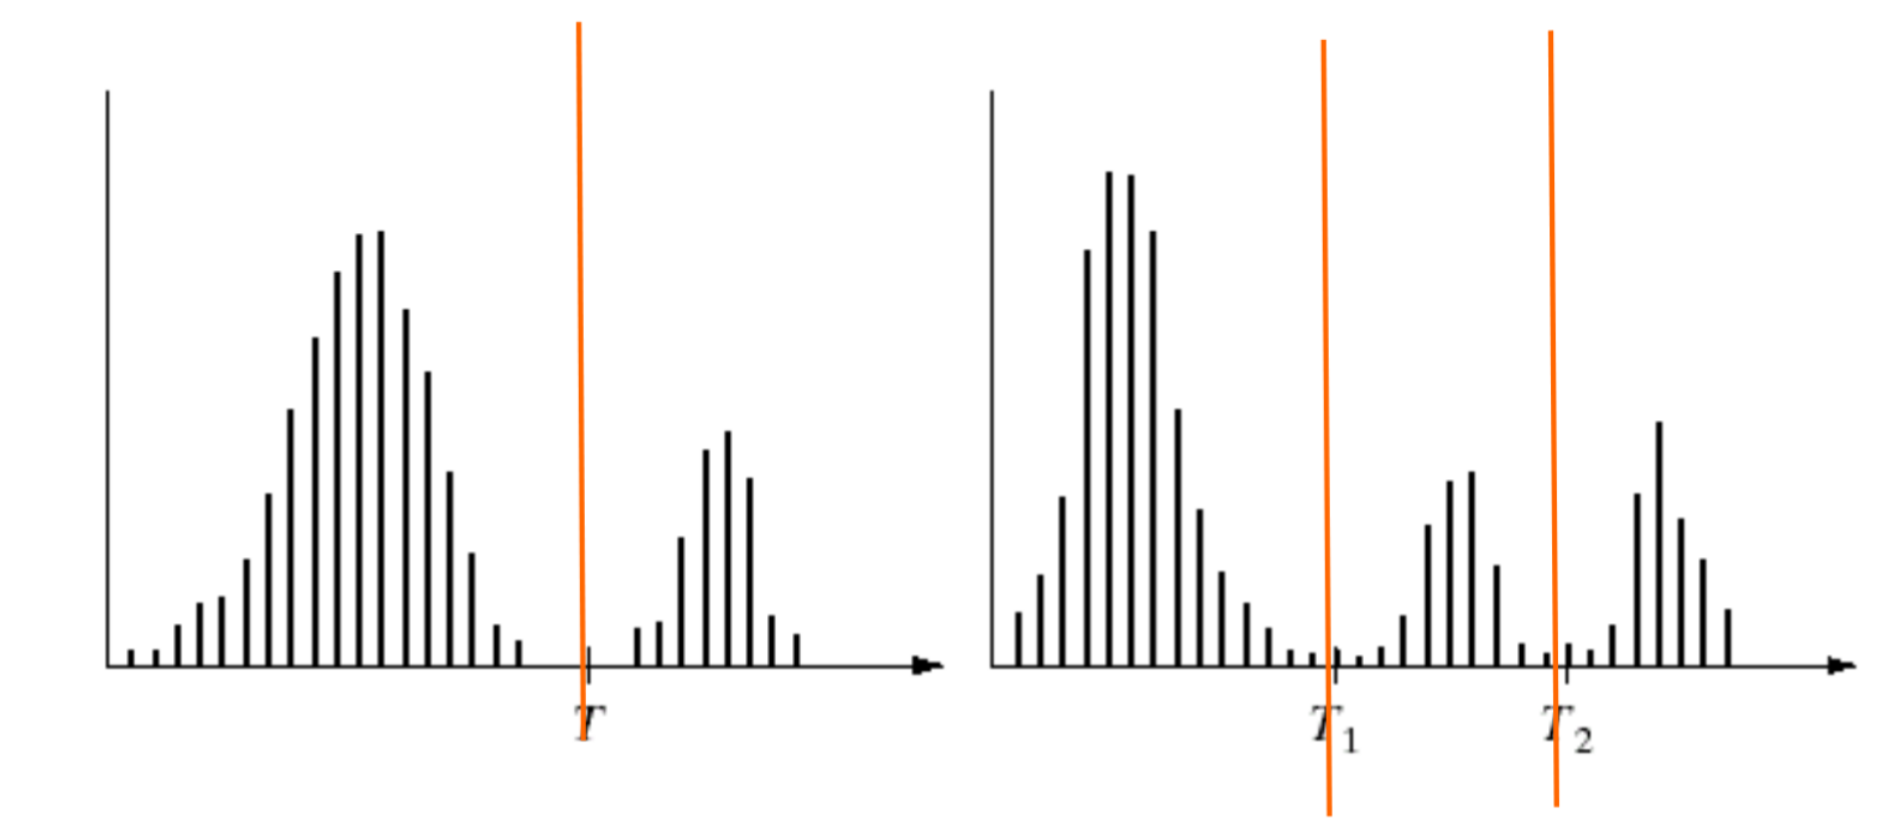
\includegraphics[width=\linewidth]{images/thresholding_histogram.png}
      \caption{Thresholding on bimodal vs. multimodal histograms}
    \end{figure}

  \item Uneven illumination can be a problem for single value thresholding.
\end{itemize}

\subsection*{Adaptive Thresholding}

\begin{itemize}
  \item For handling situations in which single value thresholding will not work
  \item Divide an image into sub images and threshold these individually
  \item Since the threshold for each pixel depends on its location within an image this technique is said to \textbf{adaptive}
\end{itemize}

